% Created 2021-01-27 Wed 14:04
% Intended LaTeX compiler: pdflatex
\documentclass[bigger]{beamer}
\usepackage[utf8]{inputenc}
\usepackage[T1]{fontenc}
\usepackage{graphicx}
\usepackage{grffile}
\usepackage{longtable}
\usepackage{wrapfig}
\usepackage{rotating}
\usepackage[normalem]{ulem}
\usepackage{amsmath}
\usepackage{textcomp}
\usepackage{amssymb}
\usepackage{capt-of}
\usepackage{hyperref}
\usetheme[progressbar=foot]{metropolis}
\author{Edmund Miller}
\date{2021-01-27 Wed}
\title{Research Update}
\hypersetup{
 pdfauthor={Edmund Miller},
 pdftitle={Research Update},
 pdfkeywords={},
 pdfsubject={},
 pdfcreator={Emacs 28.0.50 (Org mode 9.5)}, 
 pdflang={English}}
\begin{document}

\maketitle

\section{Overview of GRO-Seq pipeline}
\label{sec:orgaafcaf7}

\begin{frame}[label={sec:org8960a97}]{Global Transcription}
\begin{center}
\includegraphics[width=.9\linewidth]{/home/emiller/sync/org/roam/data/27/a69cce-9e12-465c-b8af-ced235ef4858/globaltrans.png}
\end{center}
\end{frame}

\section{Recap}
\label{sec:org8bba0b9}

\begin{frame}[label={sec:org2de6ffe}]{Overview}
\begin{itemize}
\item Reproducing GM18
\item Predicted IMR90 eRNAs
\item Compared IMR90 Predicted Enhancers to GM
\item Used Homer scripts to find DE of eRNAs and Genes
\item Gene Centric vs. Enhancer Centric
\end{itemize}
\end{frame}

\begin{frame}[label={sec:orga98513d}]{Reproducing GM18}
\begin{itemize}
\item hg18 vs hg19
\item Overpredicting eRNA transcripts
\item Past Issue
\begin{itemize}
\item What I thought Peng sent me
\item hg18 -> eRNAs -> Me
\item What actually happened
\item hg18 -> eRNAs -> LiftOver -> hg19 -> Me
\end{itemize}
\item Main issue is homer uniqmap
\end{itemize}
\end{frame}

\begin{frame}[label={sec:orgcbf22da}]{DAG of workflow}
\begin{center}
\includegraphics[height=0.7\linewidth]{/home/emiller/sync/org/roam/data/93/3abd13-dab2-4bf6-8a59-7aa16f9d6cc9/dag.png}
\end{center}
\end{frame}

\begin{frame}[label={sec:org52c8e0d}]{Enhancer Transcript Identification}
Changes from GM18
\begin{itemize}
\item hg19
\item No liftover
\end{itemize}
\end{frame}

\begin{frame}[label={sec:orge1266a4}]{IMR/GM enhancer transcript overlaps}
\begin{center}
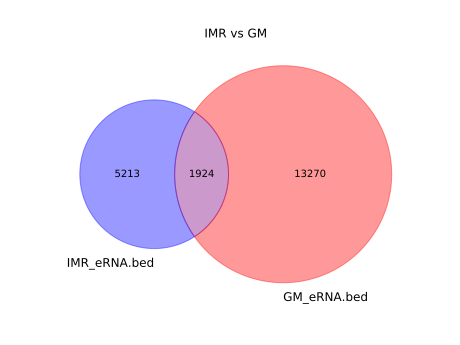
\includegraphics[width=.9\linewidth]{/home/emiller/sync/org/roam/data/d6/9b864e-96b4-481d-9b67-be5af10bac64/eRNA_cross_cell.png}
\end{center}
\end{frame}

\begin{frame}[label={sec:org14f59c5}]{IMR/GM enhancer transcripts linked to DGEs}
\begin{center}
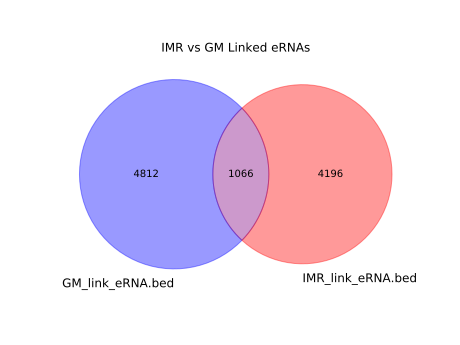
\includegraphics[width=.9\linewidth]{/home/emiller/sync/org/roam/data/4c/de863e-2a68-4676-9768-e7da5b7ba5f0/eRNA_cross_cell_viral.png}
\end{center}
\end{frame}

\begin{frame}[label={sec:org9e6577a}]{Gene Centric vs. Enhancer Centric}
\begin{itemize}
\item Peng's approach
\begin{itemize}
\item Took enhancers that were expressed deferentially
\item Linked them to Genes within 200Kb
\end{itemize}

\item New approach
\begin{itemize}
\item Find genes that are deferentially expressed
\item Link the Enhancers to those genes
\end{itemize}
\end{itemize}
\end{frame}

\begin{frame}[label={sec:org6dad36b}]{Gene Centric vs. Enhancer Centric}
\begin{center}
\includegraphics[height=0.7\linewidth]{/home/emiller/sync/org/roam/data/29/57af0c-1869-4c5a-9349-ac9205d2b7b0/enhancer_centric_pipeline.png}
\end{center}
\end{frame}

\section{nf-core}
\label{sec:org14268a6}

\begin{frame}[label={sec:org5a6b3d4}]{Standardizing Snakemake}
\begin{itemize}
\item January 2020
\item Template
\item Universal Commands
\item Testing
\item CI/CD
\item Wrappers
\end{itemize}
\end{frame}

\begin{frame}[label={sec:orgaa597db}]{nf-core Paper}
\begin{center}
\includegraphics[width=.9\linewidth]{/home/emiller/sync/org/roam/data/45/1876b4-d9c8-47e7-a0e4-76e3e6403a4a/_20210127_123601screenshot.png}
\end{center}
\end{frame}

\begin{frame}[label={sec:org6e5502c}]{nf-core Features}
\begin{center}
\includegraphics[height=0.7\linewidth]{/home/emiller/sync/org/roam/data/b9/be7b67-b57f-4f58-8cda-36455fb83c53/_20210127_123835screenshot.png}
\end{center}
\end{frame}

\begin{frame}[label={sec:org51f0943},fragile]{nf-core Getting started}
 \begin{verbatim}
# Install nextflow
curl -s https://get.nextflow.io | bash
mv nextflow ~/bin/

# Launch the RNAseq pipeline
nextflow run nf-core/rnaseq \
    --input samplesheet.csv \
    --genome GRCh37 \
    -profile docker
\end{verbatim}
\end{frame}

\begin{frame}[label={sec:org73b8698}]{nf-core Contributions}
\begin{itemize}
\item Rewriting modules that weren't dogfood
\item Added indepth testing for modules using pytest-workflow
\begin{itemize}
\item \href{https://pca.st/xdutlokp}{Testing in Scientific Research and Academia - Martin Héroux - Test \& Code : P\ldots{}}
\end{itemize}
\item Coming Soon
\begin{itemize}
\item Pytest-workflow tests for pipelines
\end{itemize}
\end{itemize}
\end{frame}

\begin{frame}[label={sec:orgfa2c0e9},fragile]{Example pytest-workflow}
 \begin{verbatim}
- name: Run fastqc paired-end test workflow
  command: nextflow run ./tests/software/fastqc/ -profile docker -entry test_paired_end -c tests/config/nextflow.config
  tags:
    - fastqc
  files:
    - path: output/test_paired_end/test_1_fastqc.html
    - path: output/test_paired_end/test_2_fastqc.html
    - path: output/test_paired_end/test_1_fastqc.zip
    - path: output/test_paired_end/test_2_fastqc.zip
\end{verbatim}
\end{frame}

\begin{frame}[label={sec:orgcbca0bd}]{nf-core Improvements to GRO-Seq pipeline}
\begin{itemize}
\item Handling of multiple genomes
\item Cluster configs
\item SRA-download
\item Plugging in down stream analysis
\end{itemize}
\end{frame}

\begin{frame}[label={sec:org20fb08e}]{Future}
\begin{itemize}
\item Adding Total Functional Score of Enhancer Elements (TFSEE) Model
\begin{itemize}
\item ChroHMM alternative
\end{itemize}
\item Integrate genomic data indicating open regions of chromatin (ATAC-seq,
DNase-seq, or MNase-seq)
\item Applying the pipeline to our datasets
\item Applying the pipeline to outside datasets
\end{itemize}
\end{frame}
\end{document}